\documentclass{article}
\usepackage{amsmath}
\usepackage{amsfonts}
\usepackage{mathbbol}
\usepackage{mathtools}
\usepackage[letterpaper,top=1in,bottom=1in,left=1in,right=1in]{geometry}
\usepackage{chngcntr}
\usepackage{amssymb}
\usepackage[verbose]{placeins}

\counterwithin*{equation}{section}
\counterwithin*{equation}{subsection}
\renewcommand{\thesubsection}{\thesection.\alph{subsection}}

\DeclarePairedDelimiter{\floor}{\lfloor}{\rfloor}
\DeclarePairedDelimiter{\ceil}{\lceil}{\rceil}
\renewcommand{\mod}{\text{ mod }}

\title{Written Assignment 9}
\author{CS 135-B/LF}
\date{April 21, 2024}

\begin{document}
\maketitle
\raggedright


\section{}
Modular arithmetic in this section is done by my code from Labs 10 and 11.\\
\begin{verbatim}
(define (mult-inv a b)
    (let ((x (cadr (pulverize a b))))
        (if (> x 0)
            x
            (+ x b))))
(define (mod-exp b e m)
    (cond
        ((= e 0) 1)
        ((= 0 (modulo e 2)) (modulo (expt (mod-exp b (/ e 2) m) 2) m))
        (else (modulo (* b (mod-exp b (- e 1) m)) m))))
\end{verbatim}
\subsection{}
"MOVE" $\rightarrow$ 1214, 2104\\
$1214^{19} \mod 7387 = 2097$\\
$2104^{19} \mod 7387 = 4767$\\
Alice will send Bob 2097 and 4767.

\subsection{}
Given $n = pq = 83\cdot89$, let $\phi = (p-1)(q-1) = 82\cdot88 = 7216$.\\
Let $d = 1899$ i.e. the multiplicative inverse of $e \mod \phi$. $d$ is Bob's private key. Given ciphertexts 2097 and 4767, we raise both to $d$ and find that value mod $n$.\\
$2097^{1899} \mod 1214 = 1214$\\
$4767^{1899} \mod 2104 = 2104$\\
1214, 2104 $\rightarrow$ "MOVE"


\section{}
No. According to page S-61 of the textbook, a complete graph $G = (V,E)$ with $|V| = n$ vertices has $|E| = n(n-1)/2$ edges. To make $|E|$ prime, one of $n$ or $n-1$ must equal 2 and the other must be prime as the 2 is divided out and results in a prime $|E|$; otherwise $|E|$ will have 2 as a factor and be composite. Since we have the bound $n>3$, the smallest $n = 4$ and $4 \neq 2$ and $4-1 = 3 \neq 2$. Therefore there is no $n>3$ than can satisfy the conditions to make $|E|$ prime. $\blacksquare$

\section{}
\begin{figure}[hbt!]
    \centering
    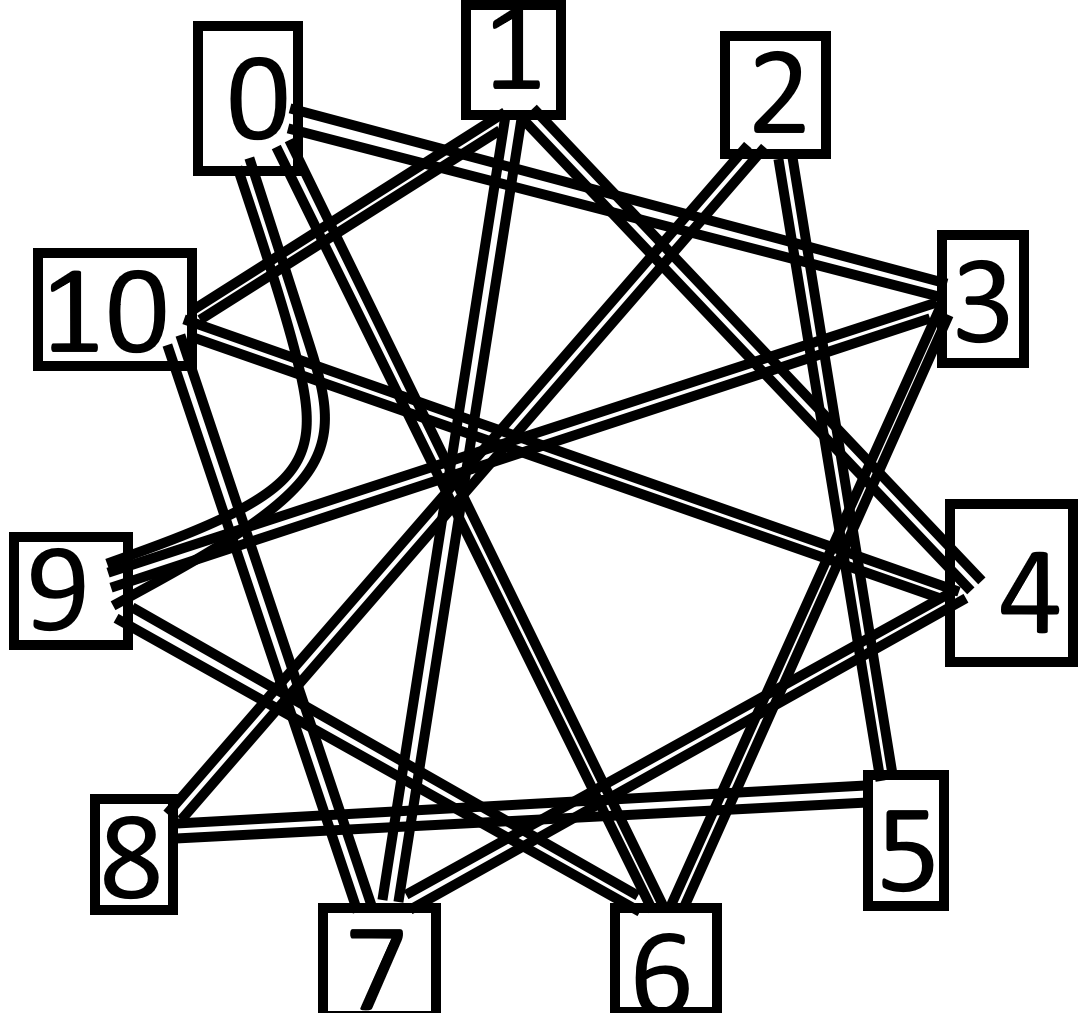
\includegraphics[width=0.7\textwidth]{graph4}
    \caption{Undirected graph $G$.}
\end{figure}

\end{document}